
\chapter{Generative Adversarial Networks (GANs)}

\begin{idea}
    One of the primary goals of GANs is to generate data that is indistinguishable from real data. This can be valuable in various applications, such as generating realistic images, videos, text, or other types of data. For example, GANs have been used to create lifelike images of nonexistent people, animals, or scenes.
\end{idea}

\section{Generative Models}

\begin{definition}
    \textbf{Generative Model:} a type of model that learns to model the probability distribution of the input data. It can generate new data points that resemble the training data, making it capable of creating synthetic data. Examples include Variational Autoencoders (VAEs) and Generative Adversarial Networks (GANs).
\end{definition}

\begin{definition}
    \textbf{Discriminative Model:} a model that learns to model the decision boundary between different classes or categories in the data. It's primarily used for classification tasks, aiming to distinguish between different classes based on input features. Examples include Logistic Regression, Support Vector Machines (SVMs), and Convolutional Neural Networks (CNNs) for image classification.
\end{definition}

\noindent \textbf{Generative Model vs. Discriminative Model}

Suppose we have two tasks on a dataset of tweets:
\begin{enumerate}
    \item Identify if a tweet is real or fake
    \begin{itemize}
        \item This task is \textbf{supervised} and requires a \textbf{discriminative model.}
        \item The model learns to approximate \textbf{$p(y|x)$}
    \end{itemize}
    \item Generate a new tweet
    \begin{itemize}
        \item This task is \textbf{unsupervised} and requires a \textbf{generative model.}
        \item The model learns to approximate $p(x)$
    \end{itemize}
\end{enumerate}

\begin{figure}[h!t]
    \centering
    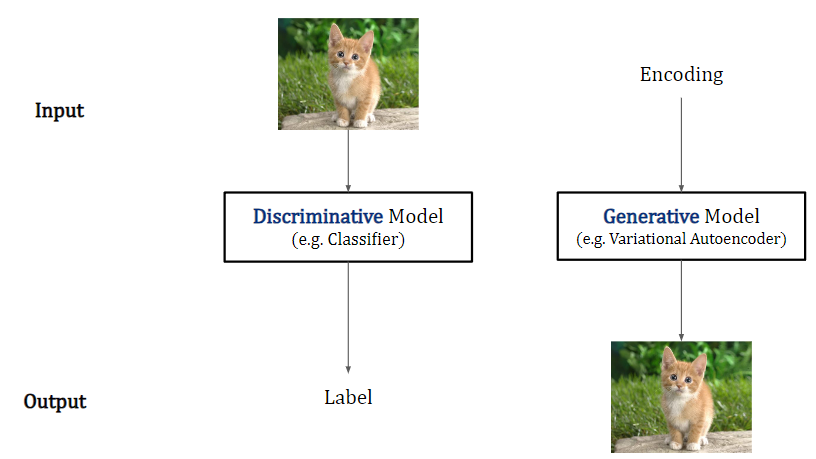
\includegraphics[width=0.8\linewidth]{gendis.png}
    \caption{Generative Model vs. Discriminative Model}
    \label{fig:enter-label}
\end{figure}
\newpage

Generative learning is an \textbf{Unsupervised Learning task}:
\begin{itemize}
    \item There is a loss function $\rightarrow$ an auxiliary task that we know the answer to
    \item There is no ground truth with respect to the actual task that we want to accomplish.
    \item We are learning the \textbf{structure \& distribution of data}, rather than labels for data!\\
\end{itemize}
\noindent \textbf{Generative Models}\\
\\A generative model is used to generate new data, using some input encoding:
\begin{itemize}
    \item \textbf{Unconditional Generative Models}
    \begin{itemize}
        \item Only get random noise as input
    \end{itemize}
    \begin{itemize}
        \item No control over what category they generate
    \end{itemize}
    \item \textbf{Conditional Generative Models}
    \begin{itemize}
        \item One-hot encoding of the target category + random noise, or
    \end{itemize}
    \begin{itemize}
        \item An embedding generated by another model (e.g., from CNN)
    \end{itemize}
    \begin{itemize}
        \item User have a high-level control over what the model will generate\\
    \end{itemize}
\end{itemize}

\\There are different families of deep generative models:
\begin{itemize}
    \item Autoregressive Models
    \item Variational AutoEncoders (VAEs)
    \item Generative Adversarial Networks (GANs)
    \item Flow-Based Generative Models (not covered in course)
    \item Diffusion Models (not covered in course)\\
\end{itemize}

\noindent \textbf{Problem with Autoencoders}\\

\begin{figure}[h!t]
    \centering
    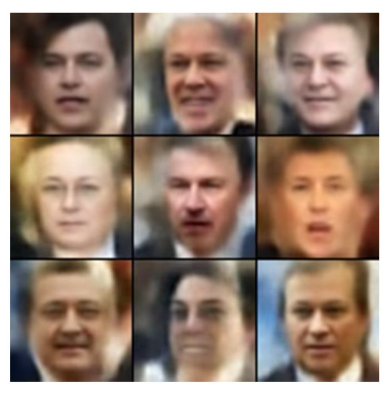
\includegraphics[width=0.4\linewidth]{blurry.png}
    \caption{Blurry result from a vanilla Autoencoder}
    \label{fig:enter-label}
\end{figure}

Vanilla autoencoders generate blurry images with blurry backgrounds. To minimize the MSE loss, autoencoders predict the average pixel (\textbf{the loss function causes the blur}). Can we use a\textbf{ better loss function}?

\section{Generative Adversarial Networks}

\begin{idea}
    \textbf{GANs:} Idea → Train two models
\end{idea}

\begin{figure}[h!t]
    \centering
    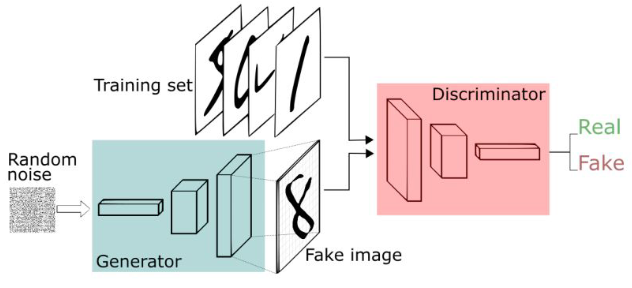
\includegraphics[width=0.775\linewidth]{gan.png}
    \caption{Architecture of a Generative Adversarial Network}
    \label{fig:enter-label}
\end{figure}

\begin{itemize}
    \item \textbf{Generator model:} try to fool the discriminator by generating real-looking images
    \item \textbf{Discriminator model:} try to distinguish between real and fake images
\end{itemize}

The loss function of the generator is defined by the discriminator!

\begin{itemize}
    \item     \textbf{Generator network}
    \begin{itemize}
        \item Input → A noise vector
        \item Output → A generated image
    \end{itemize}
    \item \textbf{Discriminator network}
    \begin{itemize}
        \item Input → An image
        \item Output → A binary label (real vs fake)\\
    \end{itemize}
\end{itemize}

\noindent \textbf{Loss Function for MinMax Game}
\begin{idea}
    In a GAN, the discriminator and generator are playing a minmax game. The discriminator is trying to do the best job it can. The generator is set to make the discriminator as wrong as possible.
\end{idea}

\begin{itemize}
    \item The \textbf{discriminator} learns weights to\textbf{ maximize the probability} that it labels a \textbf{real image as real} and a \textbf{generated image as fake}
    \item Since there are\textbf{ two possiblities} as output for the discriminator (true \& false), the optimal loss function is \textbf{Binary Cross-Entropy}
\end{itemize}

\begin{itemize}
    \item On the other hand, the \textbf{generator} learns weights to \textbf{maximize the probability} that the \textbf{discriminator labels a generated (fake) image as real}
    \item The loss function of the generator is the\textbf{ discriminator} itself
    \begin{itemize}
        \item This is because if generator wins, discriminator loses and if generator loses, discriminator wins; there are only two possible scenarios
    \end{itemize}

\end{itemize}

\textbf{Training}
\begin{itemize}
    \item \textbf{Alternate} between training the discriminator and training the generator
\end{itemize}

\begin{idea}
    GANs are notoriously difficult to train. One difficulty is that a training curve is no longer as helpful as it was for a supervised learning problem! The generator and discriminator losses tend to bounce up and down, since both the generator and discriminator are changing over time. Tuning hyperparameters is also much more difficult because we don't have the training curve to guide us.
\end{idea}

\begin{figure}[h!t]
    \centering
    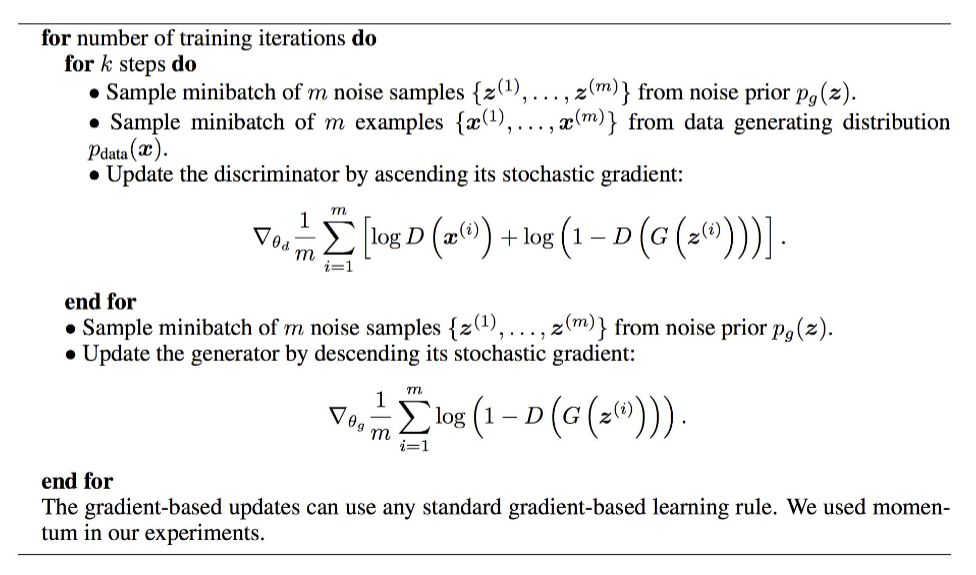
\includegraphics[width=1\linewidth]{traininggnn.png}
    \caption{Training a GAN}
    \label{fig:enter-label}
\end{figure}

\section{PyTorch Implementation}

\begin{figure}[h!t]
    \centering
    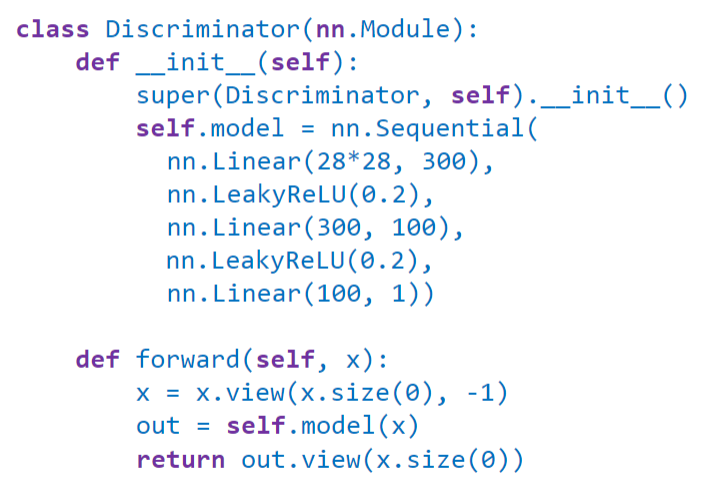
\includegraphics[width=0.6\linewidth]{discriminator.png}
    \caption{PyTorch Implementation of a Discriminator}
    \label{fig:enter-label}
\end{figure}
\begin{figure}[h!t]
    \centering
    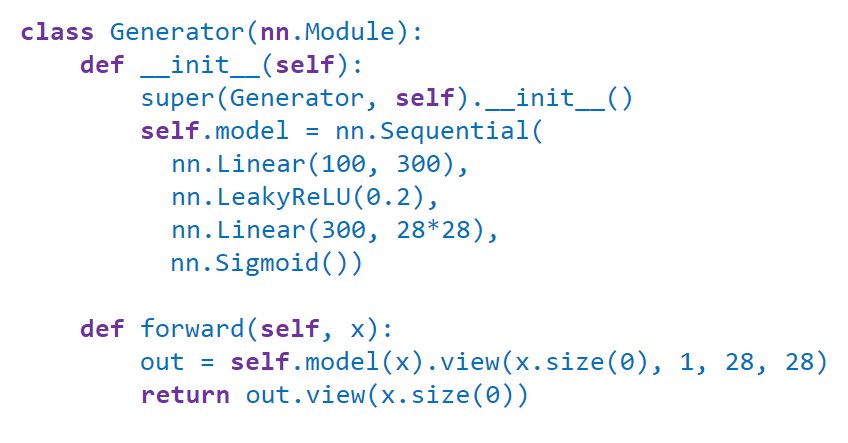
\includegraphics[width=0.75\linewidth]{generator.png}
    \caption{PyTorch Implementation of a Generator}
    \label{fig:enter-label}
\end{figure}

\begin{figure}[h!t]
    \centering
    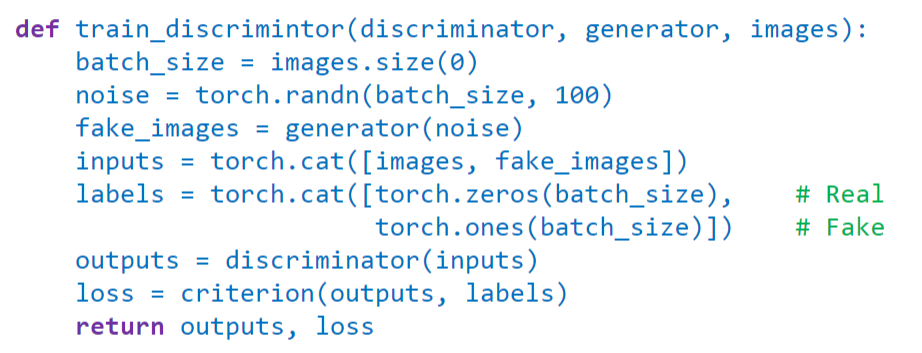
\includegraphics[width=0.75\linewidth]{trainingdiscriminator.png}
    \caption{PyTorch Implementation of Training the Discriminator}
    \label{fig:enter-label}
\end{figure}

\begin{figure}[h!t]
    \centering
    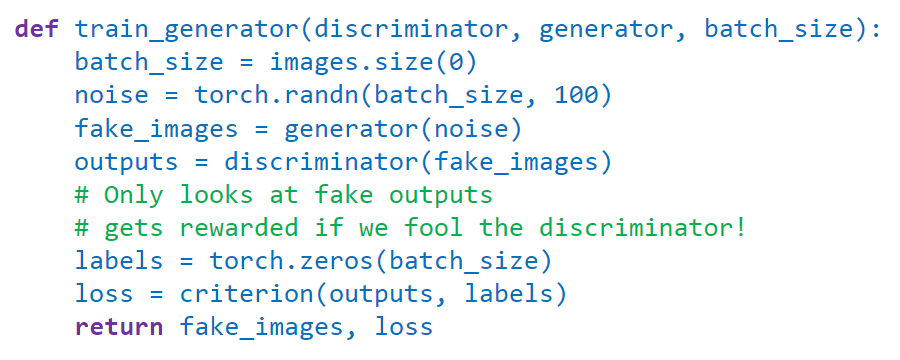
\includegraphics[width=0.75\linewidth]{traininggenerator.png}
    \caption{PyTorch Implementation of Training the Generator}
    \label{fig:enter-label}
\end{figure}

\newpage

\section{Problems of Training GANs}

\textbf{Vanishing Gradients}
\begin{itemize}
    \item If the discriminator is too good, then the generator will not learn (or the other way around)
    \item Remember that we are using the discriminator as a loss function for the generator
    \item If the discriminator is too good, small changes in the generator weights \textbf{won’t change the discriminator output}
    \begin{itemize}
        \item No proper feedback for the generator to improve
    \end{itemize}
    \item If small changes in generator weights make no difference, then we can’t incrementally improve the generator \textbf{(no gradients!)}

\end{itemize}
\noindent
\textbf{Mode Collapse}

\begin{figure}[h!t]
    \centering
    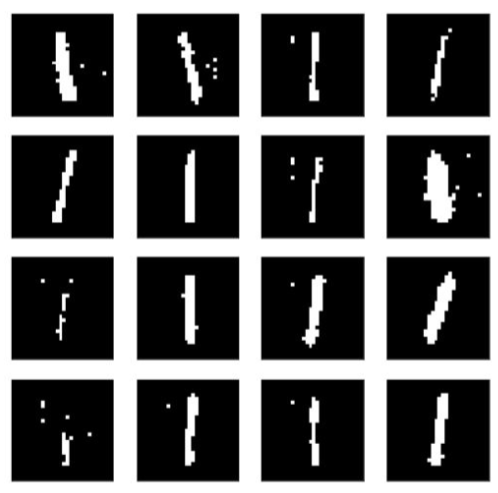
\includegraphics[width=0.2\linewidth]{modecollapse.png}
    \caption{Mode Collapse}
    \label{fig:enter-label}
\end{figure}

\begin{itemize}
    \item We want the generator to generate variety of outputs (e.g., all digits within MNIST).
    \item If generator starts producing the\textbf{ same output (or a small set of outputs),} the best strategy for the discriminator is to reject that output.
    \item However, if the discriminator is trapped in \textbf{local optimum}, it cannot adapt to generator, and the generator can fool it by only generating one type of data (e.g. only digit 1)
    \begin{itemize}
        \item Basically, the detector become very good at detecting some specific categories but not others.
        \item The generator exploits this weakness
    \end{itemize}

\begin{idea}
    To prevent mode collapse, newer variations of GANs provides the discriminator with a small set of either real or fake data, rather than one at a time. A discriminator would therefore be able to use the variety of the generated data as a feature to determine whether the entire small set of data is real or fake
\end{idea}
\end{itemize}
\noindent
\textbf{Failing to Converge}
\begin{itemize}
    \item Due to the MinMax optimization process, training Vanilla GANs is \textbf{very difficult}.
    \item It is difficult to numerically see whether there is progress → Plotting the “training curve” doesn’t help much!
    \item Takes a long time to train (a long time before we see progress)
    \item To train GANs faster, we’ll use:
    \begin{itemize}
        \item LeakyReLU Activations instead of ReLU
        \item Batch Normalization
        \item Regularizing discriminator weights \& adding noise to discriminator inputs
    \end{itemize}

\end{itemize}

\section{Applications of GANs}

\begin{itemize}
    \item \textbf{Face Generation (This Person Does Not Exist)}

\begin{figure}[h!t]
    \centering
    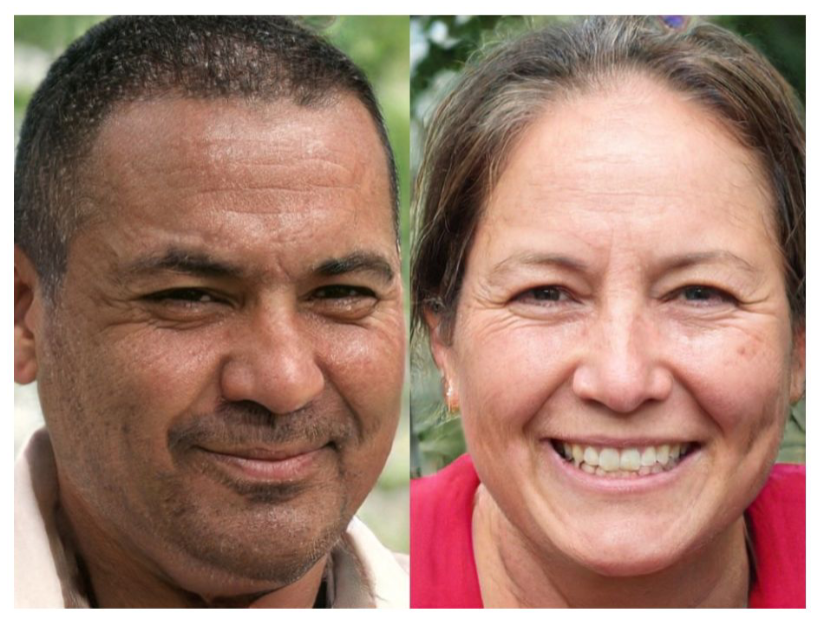
\includegraphics[width=0.1\linewidth]{facegen.png}
    \caption{Examples of GAN-generated faces}
    \label{fig:enter-label}
\end{figure}

    \item \textbf{Grayscale to Color}
\end{itemize}

\begin{figure}[h!t]
    \centering
    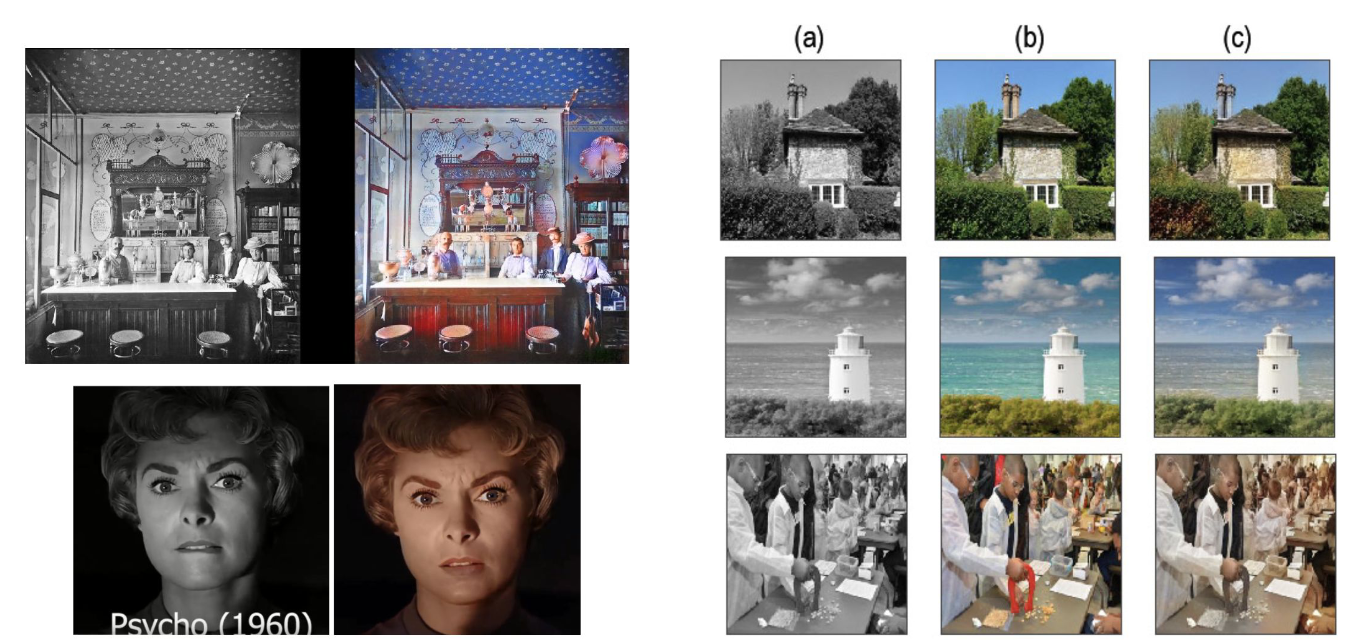
\includegraphics[width=0.35\linewidth]{grayscaletocolor.png}
    \caption{Grayscale to color examples}
    \label{fig:enter-label}
\end{figure}


\begin{idea}
    Grayscale to color involves a conditional generator.
\end{idea}

\begin{figure}
    \centering
    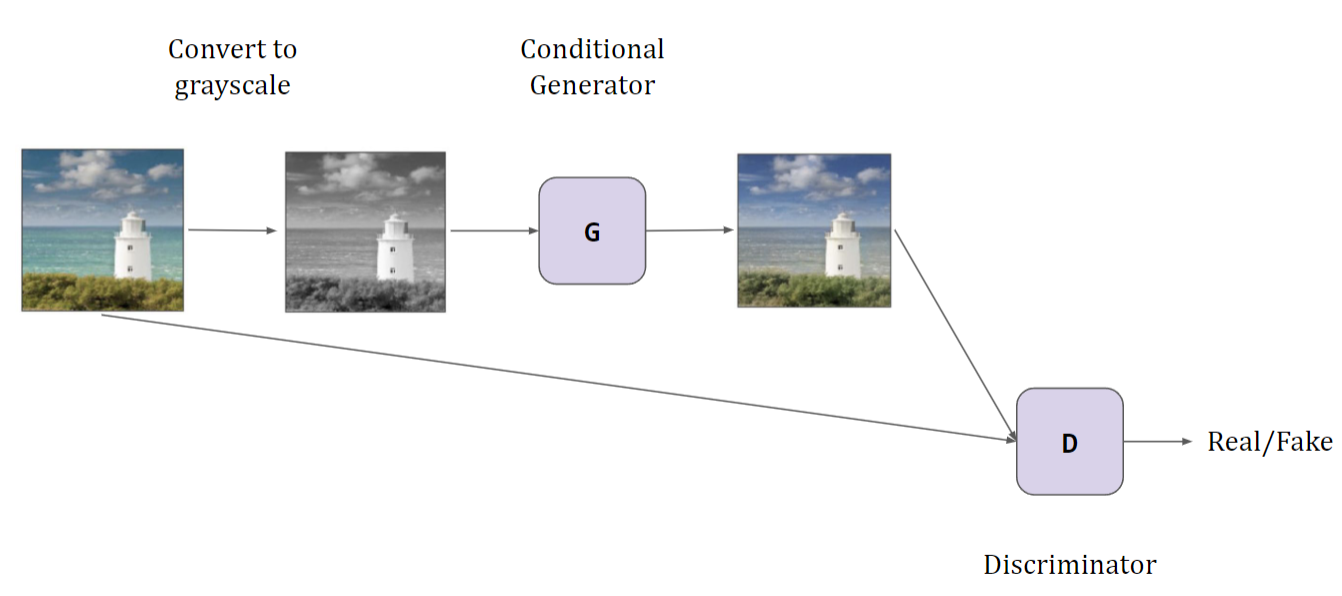
\includegraphics[width=0.75\linewidth]{condgen.png}
    \caption{Conditional Generator}
    \label{fig:enter-label}
\end{figure}

\newpage

\begin{example}

\textbf{How could we have a GAN trained on MNIST output only specific digits?}

Pass the specific class as input to the generator and discriminator so that both will know what type of class is being generated, and they can compete on that specific class

\end{example}

\begin{figure}[h!t]
    \centering
    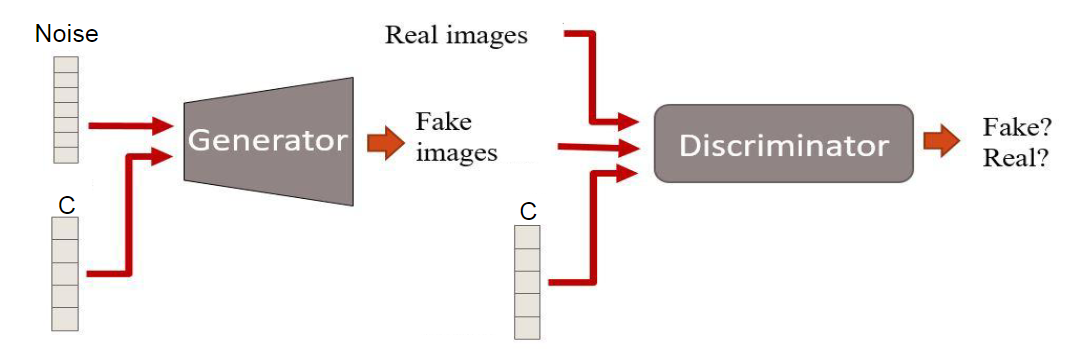
\includegraphics[width=0.75\linewidth]{mnstcongen.png}
    \caption{Passing in a specific class}
    \label{fig:enter-label}
\end{figure}

\begin{itemize}
    \item \textbf{Style Transfer}
\end{itemize}

\begin{figure}[h!t]
    \centering
    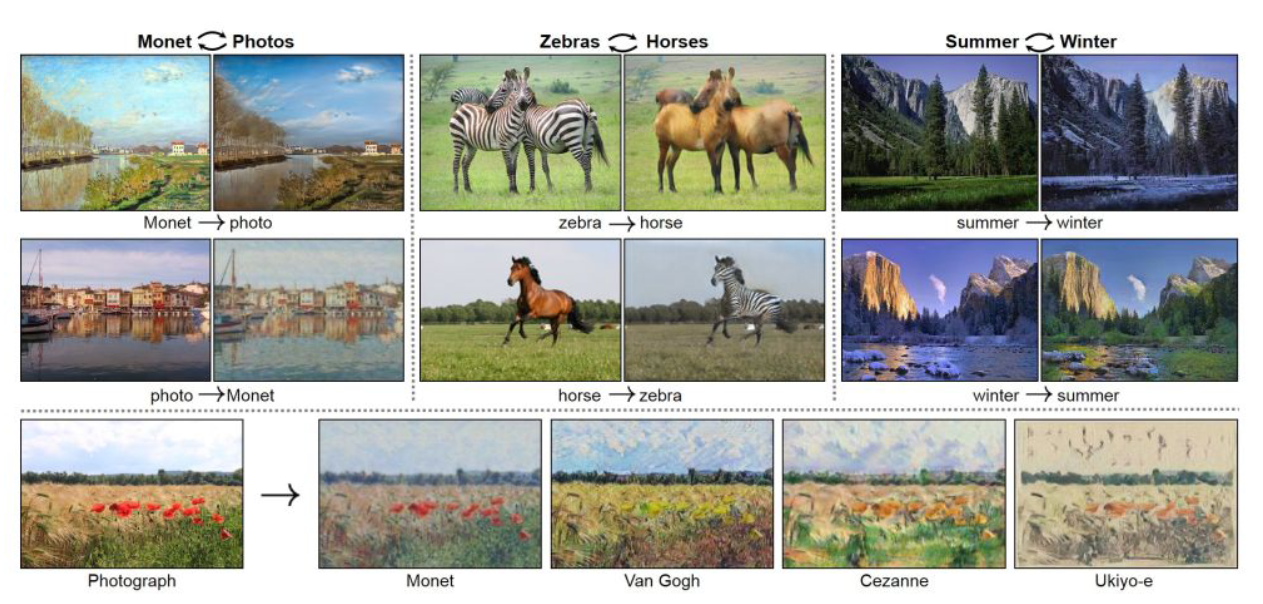
\includegraphics[width=1\linewidth]{styletransfer.png}
    \caption{Style Transfer}
    \label{fig:enter-label}
\end{figure}

\textbf{Cycle GAN:} Cycle loss is reconstruction loss between input to cyclegan and output of cyclegan to ensure consistency (consists of two gans)

\begin{figure}[h!t]
    \centering
    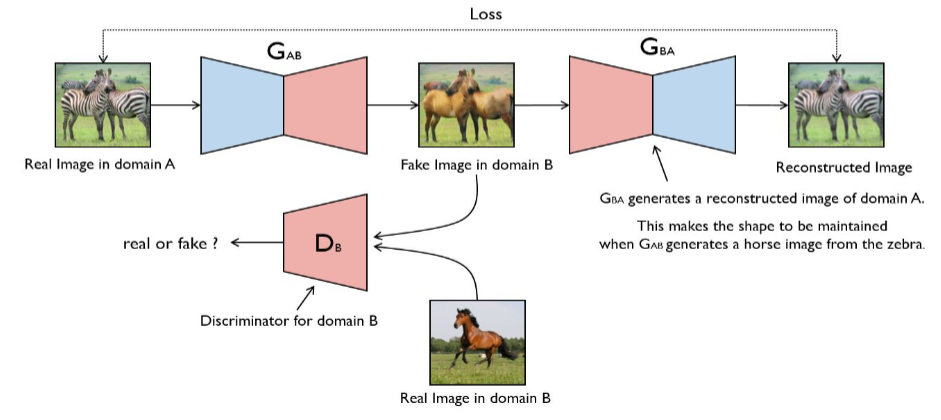
\includegraphics[width=1\linewidth]{cyclegan.png}
    \caption{CycleGan}
    \label{fig:enter-label}
\end{figure}

\newpage

\section{Adversarial Attacks}

\begin{figure}[h!t]
    \centering
    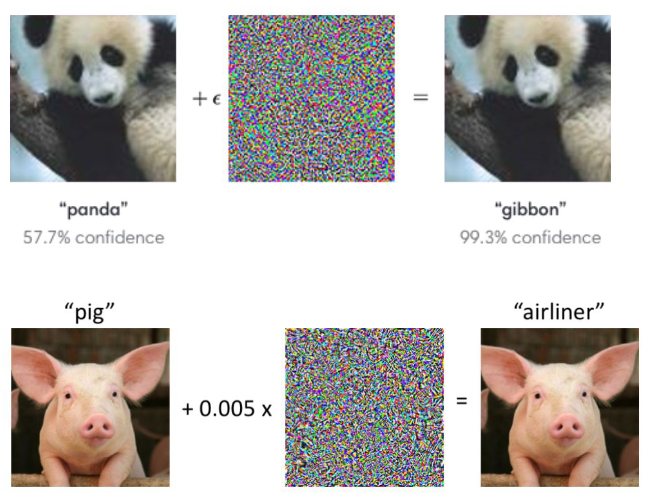
\includegraphics[width=0.75\linewidth]{adversarialexamples.png}
    \caption{Adversarial Examples}
    \label{fig:enter-label}
\end{figure}

\begin{definition}
    \textbf{Adversarial Attack:}  a deliberate manipulation of input data, typically to machine learning models, with the goal of causing the model to make incorrect predictions or classifications. These manipulations are often small, imperceptible changes designed to exploit vulnerabilities in the model's decision boundaries and undermine its accuracy and reliability. Adversarial attacks can pose a significant security and reliability challenge for machine learning systems.
\end{definition}

\begin{itemize}
    \item \textbf{Goal}: Choose a small perturbation $\epsilon$ on an image x so that a neural network f misclasses x + $\epsilon$
    \item \textbf{Approach}: Use the same optimization process to choose $\epsilon$ to minimize the probability that

\[f(x + \epsilon) = \text{correct class}\]
\item We are treating $\epsilon$ as the \textbf{parameters}


\end{itemize}

\noindent
\textbf{Targeted vs. Non-Targeted Attack}
\begin{itemize}
    \item \textbf{Non-targeted attack}
    \begin{itemize}
        \item Minimize the probability that: 
\[f(x + \epsilon) = \text{correct class}\]
\item The attacker's goal is to cause any form of misclassification or disrupt the model's predictions without specifying a particular target class
\item The objective is to \textbf{degrade the model's performance} without a specific end result in mind
\item Example: manipulate image of cat so that it's classified as anything other than a cat
\item  Often easier to carry out because they do not require the attacker to have knowledge of the target class. They may use simpler techniques and do not necessarily need to find the smallest perturbation
\end{itemize}
\item \textbf{Targeted attack}
\begin{itemize}
    \item Maximize the probability that:

\end{itemize}
\[f(x + \epsilon) = \text{target class}\]
\begin{itemize}
    \item  Attacker aims to cause a particular misclassification or a specific response from the machine learning model
    \item The attacker has a \textbf{clear target class} or outcome in mind
    \item Example: manipulate image of cat so that it's classified as a dog
    \item Requires a deep understanding of the model's decision boundaries and often involve optimization techniques to find the smallest possible perturbations that achieve the desired target outcome
\end{itemize}
\end{itemize}

\begin{idea}
    Targeted and Non-Targeted Attacks differ in the attacker's intent.
\end{idea}
\noindent
\textbf{White-Box vs. Black-Box Attacks}
\begin{itemize}
    \item \textbf{White-box attacks}
    \begin{itemize}
        \item Assumes that the model is known
    \end{itemize}
    \begin{itemize}
        \item We need to know the architectures and weights of f to optimize $\epsilon$ 
    \end{itemize}
    \item \textbf{Black-box attacks}
\begin{itemize}
    \item Don’t know the architectures and weights of f to optimize $\epsilon$
\end{itemize}
\begin{itemize}
    \item Substitute model mimicking target model with known, differentiable function
\end{itemize}
\begin{itemize}
    \item Adversarial attacks often transfer across models! (because they aren't tailored to a model with specific parameters)
\end{itemize}

\end{itemize}

\begin{idea}
    White and Black-Box Attacks differ in the attacker's knowledge of the model.
\end{idea}
\noindent
\textbf{Defence Against Adversarial Attack}\\
It is a very active area of research, and we still don’t know how to handle them. Failed Defenses:
\begin{itemize}
    \item Adding noise at test time
    \item Averaging many models
    \item Weight decay
    \item Adding noise at training time
    \item Adding adversarial noise at training time
    \item Dropout
\end{itemize}